% !TeX program = pdflatex

\documentclass{utthesis}

\usepackage{lipsum} % Dummy text for examples
\usepackage{graphicx}
\usepackage{natbib}
\usepackage{longtable}
\usepackage{amsmath, amssymb}
\usepackage{url}
\usepackage{subfigure}
%\usepackage[hidelinks,pagebackref]{hyperref} % Handy for links, can comment for plain PDF
\bibliographystyle{aasjournal}

\DeclareMathOperator\erf{erf}
\providecommand{\e}[1]{\ensuremath{\times 10^{#1}}}

\UTyear=2016

\makeindex

%\graphicspath{{./Figures/}}


\begin{document}

\author{Kevin Gullikson}
\title{Spectroscopic Detection and Characterization of Extreme Flux-Ratio Binary Systems}
\date{Revised: \today}

\UTcopyrightlegend % Optional

\begin{UTcommittee}
\UTaddsupervisor{Adam Kraus}
\UTaddcommittee{Sarah Dodson-Robinson}
\UTaddcommittee{Daniel T. Jaffe}
\UTaddcommittee{Edward L. Robinson}
\UTaddcommittee{Michael Meyer}
\end{UTcommittee}

\UTtitlepage{M.A.}{May}

\frontmatter

\setcounter{page}{4}

%\include{acknowledgements}
%\include{preface}

\begin{UTabstract}{Adam Kraus}
\lipsum[1]
\end{UTabstract}


% add . to include section numbers (non-standard)
\tableofcontents
%\tableofcontents.

\listoffigures

\mainmatter

\chapter{Introduction}

Stellar multiplicity is an inevitable and common outcome of star formation, with roughly half of all solar-type field stars in binary or multiple systems \citep{Raghavan2010} and an even higher fraction as the stellar mass increases \citep{Zinnecker2007}. Young stellar associations and clusters tend to have even higher multiplicity \citep{Duchene2013}, indicating that stars often form in multiple systems that are subsequently destroyed by dynamical interactions as the cluster dissociates. 

The overall multiplicity rate and the distributions of mass ratio, period, and eccentricity of a binary star population place important constraints on the mode of binary star formation. While the period and eccentricity are altered by dynamical processing in the birth cluster, the present-day mass ratio of a binary system is a direct result of its formation \citep{Parker2013}. Most binary stars are thought to form via core fragmentation \citep{Boss1979, Boss1986, Bate1995}, in which a collapsing core fragments into two or more individual protostars. The number and initial masses of the fragments are set by the total core mass, as well as its rotation, turbulence, and its temperature and density structure. If the fragments are well separated ($a \gtrsim 1000$ AU), they will evolve independently of each other, accreting mass from the core material onto their own protostellar disks and then onto the protostars themselves. However, close fragments ($a \sim 100$ AU) will interact with each other; the protostellar disk may be truncated, destabilized, or form into a circumbinary disk if the separation is small enough \citep{Bate1997}. In addition, an unstable disk can fragment to form low-mass companions \citep{Kratter2006, Stamatellos2011}. The mass ratios of close companions formed via either mechanism should be affected by preferential accretion. Most work has suggested that the disk material will preferentially accrete onto the lower mass companion as it migrates inward \citep{Bate1997, BBB2002}.

Intermediate-mass stars have recently seen a revival of interest as potentially young planet hosts, spurred largely by the detection of planets orbiting nearby \mbox{$\sim2 M_{\odot}$} stars on both wide \citep[e.g.][]{Lagrange2010, Marois2008} and close \citep{Johnson2011} orbits. Since the main sequence lifetime of an A- or B-type star is tens to hundreds of Myrs, a planetary companion would still be bright and easier to detect with direct imaging techniques [CITE] than the same companion orbiting an old, solar-type star. Robust age estimates for nearby intermediate-mass stars are therefore very important to convert the companion brightness into a mass estimate. 

In the context of planetary companions, stellar-mass binary companions are contaminants; companions complicate radial velocity planet searches because they necessitate simultaneous modeling of both stellar motions \citep[e.g.][]{Bergmann2015}. Likewise, companions complicate direct imaging planet searches by requiring either extremely high-contrast instrumentation \citep{Thalmann2014} or specialized coronagraphs \citep{Crepp2010}. 

However, known binary stars are typically avoided in planet search programs for a more fundamental reason: the binary companion depletes or destroys the planet-forming disk. By combining a binary census of the $\sim 2$ Myr Taurus-Auriga star-forming region with a disk census of the same, \cite{Kraus2012} showed that close ($\lesssim 40$ AU) binaries are about 2-3 times less likely to host a protoplanetary disk, and so hasten disk dispersal. Even if a disk survives, it tends to be depleted in mass by a factor of $\sim 25$ for binary separations $\lesssim 30$ AU \citep{Harris2012}. A full binary census focusing on companions within $\sim 100$ AU is therefore necessary in order to generate a direct-imaging planet search sample.

\section{Detection Methods}

There are three main main methods traditionally used to search for companions to stars, whether they be stellar or planetary companions. The first is direct imaging, in which we take an image of the star and look for nearby point sources in the image. This can be either seeing-limited, in which case it is difficult to find companions inside $1''$ of the primary, or with adaptive optics systems on large-aperture telescopes. We can detect companions out to a few hundred mas from the primary with adaptive optics imaging methods \citep[see][for typical sensitivity curves]{DeRosa2014}, and even closer with more time-consuming and complicated observational techniques such as angular differential imaging [CITE]. 

The second detection method is interferometry, in which multiple multiple beams of light from the source are allowed to constructively or destructively interfere with each other before recording the light. In some cases, interferometry is done with multiple telescopes separated by several tens of meters, producing an effective aperture much larger than can be produced as a single mirror. In other cases, a mask is introduced in front of a single telescope to only allow light from certain beams through. Interferometry can usually achieve smaller working angles than imaging, but cannot achieve as high contrast \citep[see e.g.][]{Aldoretta2015}.

The final traditional method useful in searching for stellar companions is radial velocity monitoring, in which the radial velocity of the star is measured many times over periods of years to decades. An unseen companion will cause the radial velocity of the primary star to oscillate. Unlike the previous two methods, the radial velocity method has no inner working angle; in fact, it works best at finding very close companions. The sensitivity falls off as the companion orbital separation increases, because the signal induced on the primary star decreases. The sensitivity also falls off as the number of spectral lines in the primary star spectrum falls, and as it rotation speed ($v\sin{i}$) increases. Careful radial velocity monitoring surveys are capable of detecting motion as small as $\sim 1 \mathrm{m\ s}^{-1}$ when observing slowly rotating solar-type stars \citep[e.g.][]{Wittenmyer2006, Fischer2009, Pepe2011}, but have difficulty achieving better than $\sim 1 \mathrm{km\ s}^{-1}$ when observing rapidly rotating hot stars [CITE].

Both imaging and interferometry can usually characterize the companion in a single image, provided the primary star parameters are sufficiently well-known. However, radial velocity monitoring is usually only capable of measuring the the minimum mass of the companion ($M_2\sin{i}$), and only after monitoring the system for $1-2$ orbital periods. For companions on long-period ($\sim 10$ years) orbits, it is an extremely time-consuming method. In Chapter \ref{chap:dsd}, we introduce a spectroscopic method that is capable of both detecting and characterizing close companions in single observations.


\section{Previous Observational Results}

The mass ratio, period, and eccentricity distributions are fairly well-known for solar type stars \citep{Duquennoy1991, Raghavan2010} and cooler stars \citep{Fischer1992, Delfosse2004}. Interestingly, the mass-ratio distribution appears to be invariant to separation for these stars \citep{Meyer2013}, contrary to the theoretical expectations. All of the distributions are much less certain for more massive stars. The reason for this is two-fold: first, more massive stars tend to more rare and farther away, meaning many of the companions are angularly close to the very bright primaries and difficult to detect with imaging techniques. Second, the primary stars tend to be rapid rotators, which limits radial velocity precision to $\sim 1 \mathrm{km\ s}^{-1}$. Additionally, detecting the companion spectrum suffers from the same flux-ratio difficulties as imaging methods.

Nonetheless, \citet{DeRosa2014} performed an adaptive optics imaging survey of nearby A-type stars, and found that the mass-ratio distribution is well-described by a power law with large slope, indicating a very strong preference for low-mass companions. They also found initial evidence that the mass-ratio distribution for companions inside $125$ AU has a much shallower power law slope than that of wide companions, and is consistent with flat. Their close companion subsample contained only 18 binary systems, and the result is complicated by the inherent difficulty of detecting close companions with low mass ratios in an imaging survey. 

Radial velocity monitoring surveys can detect much closer companions than imaging surveys, but are typically only complete to low-mass companions if the primary is a slow rotator. Chemically peculiar Am stars are typically associated with binary companions, and are slow rotators due to tidal braking; they thus form a highly biased sample of intermediate-mass stars. Nonetheless, it is interesting to note that they have a mass-ratio distribution which peaks near $q \sim 0.5$ \citep{Vuissoz2004}, an entirely different form than the distribution found around chemically normal stars at wide separations.


%%%%%%%%%%%%%%%%%%%%%%%%%%%%%%%%%%%%%%%%%%%%%%%%%%
% Chapter 1  (DSD method)
%%%%%%%%%%%%%%%%%%%%%%%%%%%%%%%%%%%%%%%%%%%%%%%%%%


\include{paper5}

%%%%%%%%%%%%%%%%%%%%%%%%%%%%%%%%%%%%%%%%%%%%%%%%%%
% Chapter 2 (telfit)
%%%%%%%%%%%%%%%%%%%%%%%%%%%%%%%%%%%%%%%%%%%%%%%%%%



\chapter{Correcting for Telluric Absorption: Methods, Case Studies, and the TelFit Code}
\label{chap:telfit}
This chapter was previously published \citep{Gullikson2014}. Both co-authors were my advisor at some point while I was developing this code. They helped guide the code requirements and provided a science case study for the work. Adam Kraus provided observational data for the case study.

\section{Introduction}
All ground-based astronomical spectra suffer from contamination by the Earth's atmosphere, which introduces so-called telluric lines into the spectrum. The wavelength of the telluric lines change very slightly with wind along the line of sight and pressure shifts in water lines, and the relative line strength can vary a great deal with the observatory location, weather and the airmass of the observation. The telluric lines must be removed from the spectrum to retrieve many stellar features redward of about 500 nm, which is a nontrivial task.

Often, telluric lines are removed by observing a rapidly rotating hot star (spectral type A or late B) near the same time and airmass as the target star and using it as a template for the telluric spectrum. This approach has several disadvantages: (1) it can be difficult to find a suitable standard star near the same time and airmass as the observation, so approximate corrections are made to the line strengths using Beer's law \citep{Beer1852}; (2) The water vapor content changes much more rapidly than the other absorbing species in the atmosphere, so scaling the whole empirical telluric spectrum is incorrect (3) the standard star has strong hydrogen and helium lines and weak metal lines that can further contaminate the science spectrum; (4) observing a standard star can take a significant amount of precious telescope time, especially for high signal-to-noise work.

A better solution is often to generate a theoretical telluric absorption spectrum from a line list and the observing conditions. Recently, several groups \citep{Seifahrt2011, Bertaux2013, Husser2013, Cotton2013, Gullikson2013} have used the LBLRTM code\footnote{\url{http://www.rtweb.aer.com/lblrtm_description.html}} \citep[][Line By Line Radiative Transfer Model]{Clough2005} for this purpose. However, the interface for the LBLRTM code can be difficult to learn, and can not directly fit an observed spectrum.

Telluric correction is vital to the work described in this thesis. In the optical, it allows us to use more of the spectrum to search for faint companions. Importantly, the red parts of the optical spectrum that are most affected by telluric contamination are where the primary-to-secondary flux ratio is smallest, and so where much of the companion-detecting power lies. Telluric correction is even more important in near-infrared spectra, where the contamination dominates at almost all wavelengths.

In this chapter we describe Telfit\footnote{The TelFit code documentation and installation directions can be found at \url{http://telfit.readthedocs.org/en/latest/}}, a code that acts as a wrapper to LBLRTM and allows for easy fitting of the telluric spectrum in astronomical data. We compare the results to those obtained from empiricial telluric correction in optical echelle spectra, and find that model-fitting produces similar telluric line residuals and is in fact better for dim targets or high signal-to-noise ratio work. We only demonstrate the use of TelFit in optical spectra in this work, but note that we use it to accurately remove the telluric contamination in near-infrared spectra in Chapters \ref{chap:dsd} and \ref{chap:survey}, and use an earlier version of TelFit in Chapter \ref{chap:pilot}


We describe the observations and data reduction used in this chapter in Section \ref{paper3_sec:obs}. We then describe the TelFit code and give a brief description of the telluric fitting procedure in Section \ref{paper3_sec:tellcorr}. Finally, we demonstrate the use of the TelFit code to correct several optical telluric bands in Section \ref{paper3_sec:results}. 




\section{Observations and Reduction}
\label{paper3_sec:obs}
We observed representative spectra for the early and late-type stars listed in Table \ref{paper3_tab:sample}. The A-stars HIP 20264 and HIP 25608 were observed with the CHIRON spectrograph on the 1.5m telescope at Cerro Tololo Interamerican Observatory (CTIO). This spectrograph has a spectral resolution of $R = 80000$ from $\lambda = 460 - 860$ nm, and uses 3x1 binning along the spatial direction. The data were bias-subtracted, flat-fielded, and extracted using standard IRAF tasks. The reduced spectra were wavelength-calibrated using a ThAr lamp exposure from immediately before the observation of the star. In order to reach high a signal-to-noise ratio and avoid detector saturation, we co-added 7 spectra after reduction and telluric correction (see Section \ref{paper3_sec:tellcorr}).

In addition, several M-type stars were observed with the Magellan Inamori Kyocera Echelle (MIKE) optical echelle spectrograph on the Clay telescope at Magellan Observatory as spectral type standards for a study of young stars \citep{Kraus2014}. We used the $0.7''$ slit, which yields a spectral resolution of $R = 35000$ from $\lambda = 335 - 950$ nm. The pixel scale oversamples the resolution with the $0.7''$ slit, so we used 2x binning in the spatial and spectral directions. The spectra were reduced using the CarPy pipeline \citep{Kelson2003}\footnote{\url{http://code.obs.carnegiescience.edu/mike}}. The reduced spectra were wavelength calibrated using a combination of a ThAr lamp exposure and the 760 nm telluric A band \citep[see][for details]{Kraus2014}.

TelFit can handle rapidly rotating early-type stars without preprocessing the spectra by fitting a Savitzky-Golay smoothing filter \citep{savitzky1964} as a pseudo-continuum for the telluric lines. For more feature-rich late-type stars, we remove an approximation to the stellar spectrum using the procedure below before fitting the telluric lines.

\begin{enumerate}
  \item Make an initial guess telluric spectrum with TelFit. The guess spectrum intentionally has slightly higher molecular mixing ratios than the correct values so that it over-corrects the telluric lines.
  \item Divide the observed spectrum by the guess telluric spectrum. This leaves a spectrum with stellar lines in absorption and telluric residuals appearing like emission lines.
  \item Find the best-fit stellar model to the absorption lines using a grid of PHOENIX model spectra \citep{Hauschildt1999} with effective temperature and log(g) near the expected values for the star.
  \item Divide the original data (before the telluric over-correction in step 1) by the best-fit normalized stellar spectrum. This leaves a spectrum that is mostly telluric lines, but which may have strong stellar line residuals.
  \item Enumerate the wavelength ranges that are strongly affected by stellar line residuals, and tell TelFit to ignore them. We ignored all wavelengths from 817.5 - 820 nm in our M-star spectra, which have strong residuals from the sodium lines.
\end{enumerate}

The fit to the primary star does not need to be perfect. Indeed, if we could perfectly model stellar spectra there would be little reason to observe them! The purpose of the preprocessing described above is to ensure that telluric lines dominate the spectrum before fitting. Any strong residuals from that process can and should be ignored in the telluric fit. While a physically better solution would be to fit the stellar and telluric spectra simultaneously, the method described above will often work well enough  for most purposes and is much faster than a simultaneous fit.


\begin{table}
  \centering
  \caption{Observations used in this paper. }
  \begin{tabular}{|ccccccc|}
  \hline
    Star &    R   &  $\mathrm{K_s}$ & SpT  & UT date  & Spectrograph & SNR    \\
         &  (mag) & (mag)      &      & yyyymmdd &              & @820 nm \\ 
    \hline \hline
    
    GJ 83.1  &  10.94  &  6.65  &  M4.6  &  20120902  &  MIKE  &  200  \\
    GJ 109 &  9.49  &   5.961   & M3.0 & 20120902 & MIKE        & 219 \\
    GJ 173  &  9.33  &  6.09  &  M1.6  &  20130203  &  MIKE  &  166 \\
    GJ 273  &  8.70  &  4.86  &  M3.6  &  20130204  &  MIKE  &  215\\
    GJ 447  &  9.86  &  5.65  &  M4.0  &  20130203  &  MIKE  &  324 \\
    GJ 581  &  9.46  &  5.84  &  M2.6  &  20130202  &  MIKE  &  336 \\
    GJ 628 &  8.92  &  5.08  &  M3.0  &  20120716  &  MIKE  &  346 \\
    GJ 908  &  8.03  &  5.04  &  M1.0  &  20120717  &  MIKE  &  328 \\
    HD 33793  &  7.90  &  5.05  &  M1.0  & 20130203  &  MIKE  &  315 \\
    HIP 20264  &  5.38  &  5.33 &  A0.0  &  20140301  &  CHIRON  &  167 \\
    HIP 25608  &  5.54  &  5.50  &  A1.0  &  20140301  & CHIRON  &  214 \\
    \hline
  
  \end{tabular}
  \label{paper3_tab:sample}

\end{table}



\section{Telluric Fitting Method}
\label{paper3_sec:tellcorr}

The TelFit code performs a least-squares fit using a constrained Levenberg-Marquardt algorithm \citep{Marquardt1963}. It is extremely flexible; the user can decide which atmospheric parameters to fit, which spectral regions to use in the fit, how the detector point spread function (PSF) is modeled, the order of the continuum fit used in each iteration, and whether the data wavelengths are calibrated to fit the model or vice versa. The algorithm will optimize the fitting variables, as well as the detector resolution and the wavelength solution. LBLRTM requires an atmosphere profile giving the temperature, pressure, and the abundance of several molecules as a function of height. We provide a default atmosphere profile\footnote{The default atmosphere profile was developed for the Michelson Interferometer for Passive Atmospheric Sounding (MIPAS) spacecraft, are is available from \url{http://www-atm.physics.ox.ac.uk/RFM/atm/}} with the TelFit code that is acceptable for mid-latitude observatories, but provide the ability to easily give an alternate atmosphere profile for more accurate results. 

While TelFit explicitly fits the temperature, pressure, and abundances at the observatory altitude, it scales the quantities at \emph{all} atmosphere layers. For the pressure and temperature, it finds the difference between the requested pressure (temperature) at the requested altitude, and the pressure (temperature) in the atmosphere profile. If $P_r$ is the requested pressure at altitude $z$, and the atmosphere profile pressure is $P_0 $ at that altitude, then the pressure $P_i $ at each atmosphere layer $z_i$ is scaled as
\begin{equation*}
  P_i \rightarrow P_i - (P_r - P_0) e^{\frac{-(z_i - z)^2}{2\cdot (10 \mathrm{km})^2}}
\end{equation*}
The temperature is scaled in the same way as the pressure above, and is done in this way so that the quantities more than about 10 km above the observatory are effectively unchanged. The mixing ratio of all molecules is scaled in a much simpler way: if $A_r$ is the requested mixing ratio at the telescope altitude, and $A_0$ is the mixing ratio in the atmosphere profile, the mixing ratio at each layer $A_i$ is given by
\begin{equation*}
  A_i \rightarrow A_i  \frac{A_r}{A_0}
\end{equation*}
\emph{Because of the way TelFit scales the temperature, pressure, and molecular mixing ratios in every atmosphere layer, the optimized values should not be taken as a measurement of the actual surface mixing ratios.}

In each iteration for the main variables (temperature, pressure, telescope zenith angle, and molecular abundances), TelFit refines the wavelength solution and detector resolution. The wavelength fitter performs a third-order polynomial fit to adjust the wavelengths of the model such that the telluric lines match the data. Alternatively, the data wavelengths can be adjusted to fit the model. The wavelength solution of the data should be very close, as TelFit will not shift any wavelengths by more than 0.1 nm. By default, TelFit fits the spectrograph PSF as a gaussian, and fits the detector resolution by finding the best gaussian width to convolve the model against. Alternatively, TelFit can do a nonparametric fit to the spectrograph PSF using the singular value decomposition described in detail in \cite{Rucinski1999}


\section{Results}
\label{paper3_sec:results}

We fit the spectra for the rapidly-rotating A0V star HIP 20264 with a two-step approach. In the first step, we fit the observatory temperature and humidity in the echelle orders dominated by the water bands at 590 nm, 650 nm, 700 nm, and 730 nm. For the rest of the fit, the humidity and temperature were fixed at the $\chi^2$-weighted average of the fits for each band. Next, we fit the $O_2$ abundance with the $\gamma$ and B bands near 630 nm and 690 nm, respectively. Because the blue end of the B band is extremely strong and absorbs nearly all the light, we only use the red half in the fit. The $O_2$ abundance was fixed at the $\chi^2$-weighted average of the individual fitted values for the two echelle orders. We then applied the best-fit parameters to every echelle order, allowing the fitter to adjust the model wavelengths and detector resolution separately for each order. For all telluric fits in this paper, we adjusted the temperature, pressure, and water vapor atmosphere profile with sounding data from the Global Data Assimilation System (GDAS) meteorological archive\footnote{The GDAS archive is available starting in December 2004 at \url{http://ready.arl.noaa.gov/READYamet.php}. Instructions for its use are included in the code documentation.}. As stated in Section \ref{paper3_sec:obs}, we fit each frame of HIP 20264 separately, and co-added the telluric-corrected spectra. The fitted value of the relative humidity varied from $18.7\%$ to $22.1\%$, and the airmass of the star increased from 1.15 to 1.52 (a change of $19^{\circ}$ in zenith angle) over the course of the 7 frames, making the individual fits crucial.

We show the telluric correction for the observation of the A0V star HIP 20264 in four water bands and two $\mathrm{O_2}$ bands in Figures \ref{paper3_fig:bstarcorr_water} and \ref{paper3_fig:bstarcorr_oxygen}, respectively. The telluric model shown is the average telluric model of the 7 individual exposures, since we corrected each one separately to better account for the changing water vapor content and telescope zenith angle. We apply a Savitzky-Golay smoothing filter to the corrected data to remove any broad features in the stellar spectrum. The water features are corrected to near the noise level of the spectrum, with the exception of the very strong telluric water band near 730 nm. The poor correction may be due to a slightly incorrect temperature and water-vapor atmospheric profile, which causes the line profile to change appreciably for strong lines. In addition, small errors in the line strength parameters are more noticable for strong telluric lines. The correction in the $\mathrm{O_2}$ B and $\gamma$ bands (Figure \ref{paper3_fig:bstarcorr_oxygen}) is somewhat worse. The same $\mathrm{O_2}$ mixing ratio undercorrects the $\gamma$ band and slightly overcorrects the B band. This systematic error may be from incorrect line strengths in the HITRAN database for the two bands. 

We observed the A1V star HIP 25608 30 minutes after HIP 20264 and at similar airmass, and so use it as a telluric standard star to directly compare our method to the empirical telluric correction method. To have comparable S/N ratios as in Figures \ref{paper3_fig:bstarcorr_water} and \ref{paper3_fig:bstarcorr_oxygen}, we co-added all 7 frames of both the the target star (HIP 20264) and the standard star (HIP 25608). We account for the different column density of absorbers in the target and standard star observations using Beer's law \citep{Beer1852} as follows. For each order, we scaled the normalized flux of the standard star ($f_s$) with

\begin{equation}
f_s \rightarrow f_s^{\gamma}
\label{paper3_eqn:correction}
\end{equation}

where $\gamma$ is determined using the normalized flux of the standard star and target star ($f_t$) and is defined as

\begin{equation}
\gamma = \text{median} \left( \frac{\log{f_t}}{\log{f_s}} \right)
\label{paper3_eqn:scale}
\end{equation}

In Equation \ref{paper3_eqn:scale}, we only use the points with $f_t < 0.95$ in the median computation, so that the noise does not dominate in the orders with few telluric lines. These empirical telluric corrections are shown in the top row of Figure \ref{paper3_fig:bstarcorr_empirical}. The corrections are quite poor in this case, mostly because the airmass of the target (standard) star changes from 1.15-1.52 (1.31-1.86) from the first to last frame, and co-adding the spectra amounts to a flux-weighted average over airmass that the correction in Equation \ref{paper3_eqn:correction} cannot capture. 

We also test an empirical telluric correction using only the last frame of the target star and the first frame of the standard star, and show the result in the bottom row of Figure \ref{paper3_fig:bstarcorr_empirical}. In this case, the airmass can be treated as approximately constant and Equation \ref{paper3_eqn:correction} does a much better job in accounting for the small airmass difference between the target and standard star spectra, with the exception of the nearly saturated oxygen lines (bottom left panel). The water line correction results in similar line residual amplitudes to the telluric modeling method (see Figure \ref{paper3_fig:bstarcorr_water} for comparison).


We now turn to a more typical-use case for the TelFit code: correcting the telluric lines in late-type stars near a feature of interest. For this, we use a series of M-type stars (see Table \ref{paper3_tab:sample}) with observations near the 819 nm sodium doublet, which is used as a gravity-sensitive age indicator for late-type stars \citep{Slesnick2006}. As the stellar age and therefore surface gravity increases, the line strength increases. Amongst main sequence M-stars, later spectral types have higher surface gravity and so we expect the equivalent width of the sodium lines to increase as we go towards later spectral types. 


Figure \ref{paper3_fig:mtellcorr} shows the telluric correction for the M1V star GJ 908. For this and all M-star spectra in this work, we fit the water vapor, temperature, and $O_2$ mixing ratio at the same time for the spectral order covering 819 nm. The bottom panel of Figure \ref{paper3_fig:mtellcorr} shows that each of the spectral lines after telluric correction come from the star itself, and that the telluric contamination is reduced to near the noise level of the spectrum. Importantly, the telluric lines that fall within the sodium doublet line profile no longer affect the profile shape. We can now directly compare the line profile of the sodium doublet lines as a function of spectral type, without the influence of telluric lines. Figure \ref{paper3_fig:lineprofile} shows the evolution of the doublet lines. The central depth stays about the same throughout the sequence, but the later spectral type stars show significantly broader line wings, leading to the known sequence in equivalent width \citep{Slesnick2006}. The robust recovery of the sodium line strengths and profiles demonstrate that TelFit can accurately remove telluric lines, even in feature-rich spectra. 


\section{Conclusions}
\label{paper3_sec:conclusion}
We presented the TelFit code, an object-oriented Python code capable of accurately fitting the telluric spectrum in ground-based spectra. We use a high signal-to-noise ratio echelle spectrum of the A0V star HIP 20264 to demonstrate the fit quality in Figures \ref{paper3_fig:bstarcorr_water} and \ref{paper3_fig:bstarcorr_oxygen}. Contrary to expectation, the water lines are typically fit to much higher precision than the $\mathrm{O_2}$ telluric lines. This is likely coming from a systematic error in the HITRAN line strength database, since the same $O_2$ mixing ratio overfits the B band and underfits the $\gamma$ band. We compare our code to an empirical telluric correction of HIP 20264, and find that the model is at least as accurate. In fact, TelFit is significantly more accurate than the empirical method when several frames of both the target and standard star are co-added.

We also demonstrated the use of TelFit for in-depth analysis of spectral features in late-type stars with a series of M-star observations near the 819 nm sodium doublet. The telluric lines were removed to near the noise level of the observations, allowing for analysis of the sodium line profiles and recovery of the known sequence of increasing equivalent width with later spectral types. Regions contaminated by telluric lines are often ignored in optical spectral analysis; accurate correction of telluric features could help open these regions up for further analysis.

This code was mostly developed and tested for correction of optical spectra. However, an early version of this code was used in \cite{Gullikson2013} to correct for telluric methane absorption in B-star spectra, with similar line residuals to those that \cite{Seifahrt2011} found in the same spectral region. We encourage the use of TelFit for correcting telluric absorption in near-infrared as well as optical data.

We would like to thank Andreas Seifahrt for his help in the early stages of code development. This project was funded by a UT Austin Hutchinson fellowship to Kevin Gullikson and start-up funding to Sarah Dodson-Robinson from the University of Texas. This work makes use of Astropy, a community-developed core Python package for Astronomy \citep{Astropy}, as well as SciPy, NumPy \citep{Oliphant2007}, and of course LBLRTM. We would like to thank the developers of all of those packages.


%%%%%%%%%%%%%%%%%%%%%%%%%%%%%%%%%%%%%%%%%%%%%%%%%%
%%%%%%%              Figures                 %%%%%
%%%%%%%%%%%%%%%%%%%%%%%%%%%%%%%%%%%%%%%%%%%%%%%%%%

%--------------------------------------------------------------------------------------


\begin{figure}
\begin{center}
\subfloat{\includegraphics[width=0.4\textwidth, height=0.23\textheight]{Figures/paper3_BstarCorr_590nm.pdf}} 
\subfloat{\includegraphics[width=0.4\textwidth,height=0.23\textheight]{Figures/paper3_BstarCorr_650nm.pdf}}
\\
\noindent 
\subfloat{\includegraphics[width=0.4\textwidth, height=0.23\textheight]{Figures/paper3_BstarCorr_700nm.pdf}} 
\subfloat{\includegraphics[width=0.4\textwidth,height=0.23\textheight]{Figures/paper3_BstarCorr_730nm.pdf}}
\caption{Correction of the water bands in optical spectra. All spectra are of the A0V star HIP 20264, and are smoothed with a Savitzky-Golay filter after telluric correction to remove any broad features in the stellar spectrum. The top panel of each figure shows the observed spectrum (black solid line) and the best-fit telluric model (red dashed line), and the bottom panel shows the residuals after division by the telluric model. The telluric water lines are corrected to very near the noise level of the spectrum in the top row, revealing weak interstellar Na D lines (top left). The telluric correction leaves residuals on the order of $5\%$ of the continuum for strong telluric lines (bottom right), possibly due to an incorrect atmosphere profile for water vapor.}

\label{paper3_fig:bstarcorr_water}
\end{center}
\end{figure}


%--------------------------------------------------------------------------------------

\begin{figure}
\begin{center}
\subfloat{\includegraphics[height=0.33\textheight]{Figures/paper3_BstarCorr_630nm.pdf}}
\\ 
\subfloat{\includegraphics[height=0.33\textheight]{Figures/paper3_BstarCorr_690nm.pdf}}
\caption{Correction of the $\mathrm{O_2}$ bands in optical spectra. All spectra are of the A0V star HIP 20264, and are smoothed with a Savitzky-Golay filter after telluric correction to remove any broad features in the stellar spectrum. The top panel of each figure shows the observed spectrum (black solid line) and the best-fit telluric model (red dashed line), and the bottom panel shows the residuals after division by the telluric model. }

\label{paper3_fig:bstarcorr_oxygen}
\end{center}
\end{figure}

%--------------------------------------------------------------------------------------

\begin{figure}
\begin{center}
\subfloat{\includegraphics[width=0.4\textwidth,height=0.23\textheight]{Figures/paper3_Empirical_690nm.pdf}}
\subfloat{\includegraphics[width=0.4\textwidth,height=0.23\textheight]{Figures/paper3_Empirical_730nm.pdf}}
\\ 
\subfloat{\includegraphics[width=0.4\textwidth,height=0.23\textheight]{Figures/paper3_Empirical_LowSN_690nm.pdf}}
\subfloat{\includegraphics[width=0.4\textwidth,height=0.23\textheight]{Figures/paper3_Empirical_LowSN_730nm.pdf}}
\caption{Empirical telluric corrections. \emph{Top Row}: Correction at high S/N ratio, where all 7 frames of both the target star (HIP 20264, A0V) and the telluric standard star (HIP 25608, A1V) were co-added before the telluric correction. In this case, both the humidity and the airmass are changing throughout both exposures and the empirical telluric correction is very poor. \emph{Bottom Row}: Correction between the last frame taken of the target star and the first frame of the standard star, a more common mode of empirical correction. In this case, the empirical telluric correction is comparable to the model fitting method presented in this paper. The left column should be compared to the bottom panel in Figure \ref{paper3_fig:bstarcorr_oxygen}, and the right column should be compared to the bottom right subfigure in Figure \ref{paper3_fig:bstarcorr_water}. The poor correction in the oxygen band (lower left panel) is the result of the slight airmass difference between the science and standard stars. The correction in equation \ref{paper3_eqn:correction} is only valid for weak or moderate lines, and does not work as well for the nearly saturated lines shown here. The empirical correction under-corrects the line core while over-correcting the wings.}

\label{paper3_fig:bstarcorr_empirical}
\end{center}
\end{figure}


%--------------------------------------------------------------------------------------


\begin{figure}[ht]
  \centering
  \subfloat{\includegraphics[height=0.33\textheight]{Figures/paper3_GJ908_Telluric.pdf}}
  \\
  \subfloat{\includegraphics[height=0.33\textheight]{Figures/paper3_GJ908_Stellar.pdf}}
  \caption{\emph{Top}: The observed spectrum of GJ 908 (black solid line) with the best-fit telluric spectrum (red dashed line) overplotted. There are telluric lines within the sodium doublet line profiles which affect any line shape measurements if they are not corrected. \emph{Bottom}: The telluric-corrected spectrum of GJ 908 (black solid line) with a PHOENIX model spectrum (red dashed line) overplotted to guide the eye. The model spectrum has the following parameters: $\mathrm{T_{eff}} = 3700 K$, $\log g = 4.0$, and $\mathrm{[Fe/H]} = -0.5$, and has been convolved with a gaussian to match the detector resolution. All of the remaining absorption lines in the spectrum come from the star.}
  
  \label{paper3_fig:mtellcorr}
\end{figure}

%--------------------------------------------------------------------------------------

\begin{figure}[ht]
  \centering
  \includegraphics[width=\columnwidth]{Figures/paper3_SodiumLineProfile_BW.pdf}
  \caption{The evolution of the sodium doublet line profile with spectral type for a series of main-sequence M-type stars. The later spectral types show significantly broader line wings.}
  \label{paper3_fig:lineprofile}
\end{figure}




%%%%%%%%%%%%%%%%%%%%%%%%%%%%%%%%%%%%%%%%%%%%%%%%%%
% Chapter 3 (Ps1 Dra A search)
%%%%%%%%%%%%%%%%%%%%%%%%%%%%%%%%%%%%%%%%%%%%%%%%%%


\include{paper4}

%%%%%%%%%%%%%%%%%%%%%%%%%%%%%%%%%%%%%%%%%%%%%%%%%%
% Chapter 4 (IGRINS simulation)
%%%%%%%%%%%%%%%%%%%%%%%%%%%%%%%%%%%%%%%%%%%%%%%%%%




\chapter{Future Direct Spectroscopic Detection of Hot Jupiters with IGRINS}
\label{chap:hotjup}
Several authors have used a variant of the method we described in  Chapter \ref{chap:psi1dra} to search for emission from ``Hot Jupiter`` planets orbiting a sun-like star. In this case the flux ratio is much more extreme, but still possible with enough high signal-to-noise ratio spectra. In this chapter, we generate simulations of the IGRINS instrument to assess whether it can detect Hot Jupiter emission. This chapter was previously published \citep{Gullikson2013}. The co-author, Mike Endl, was my co-supervisor at the time and provided much of the inspiration for the work as well as a great deal of technical assistance. While the instrument was being built at the time of publication, it is now functioning on the 2.7m telescope at McDonald Observatory and a pilot survey based on this work is in progress.


\section{Introduction}
With about 1600 confirmed extrasolar planets \citep[from
exoplanets.org:][]{exoplanet}, the time for characterization of these
planets is here. A first step towards characterization is a determination of
the planet mass. Most of the exoplanets so far discovered around nearby stars were
found using the radial velocity technique, which measures the periodic
Doppler shift of the parent star. Unfortunately, the inclination of the orbit cannot be determined
without another complementary method. This means that planet masses from
radial-velocity surveys are only \emph{minimum} masses. In principle, precise astrometry could provide the complementary measurement that is needed to determine the true planet mass. However, the astrometric motion is very difficult to detect with current technology. The amplitude of the motion of a sun-like star with a Jupiter-mass planet orbiting at 0.1 AU and a distance from Earth of 10 pc is roughly $20 \mu$as, an order of magnitude below the precision of the Hubble Space Telescope Fine Guidance Sensors \citep{Benedict2006} and will be very near the precision of GAIA \citep{Sozzetti2001}.

We can measure the true mass and inclination of a planet only if the
radial velocity of the planet was known as well as that of its parent
star. There are two ways that the
radial velocity of an orbiting planet could be measured: light
reflected from the parent star or the characteristic spectrum of the planet itself. Both methods require high resolution spectroscopy in order to detect the doppler motion of the spectral lines. Several groups have
attempted to detect the reflected light from orbiting planets, but at
the time of this writing none have been successful \citep{Collier2002,
  Rodler2008, Rodler2010, Langford2011} and have only been able to set upper limits on the planet albedo ($A_B \sim 0.1
$).

While searches for reflected light are best done in the optical, the
thermal emission from a $\sim 1000$K planet will peak in the
near-infrared. The thermal emission from a small group of planets has been detected,
including HD209458b \citep[e.g.][]{Knutson2007, Swain2008,
  Cubillos2010}, HD189733b \citep[e.g.][]{Grillmair2007, Knutson2007_2,
  Char2008, Agol2010}, Wasp-3b \citep{Zhao2012}, and even the
Super-Earth 55 Cnc b \citep{Demory2012}. These detections were mostly made
using either Spitzer photometry or low-resolution spectroscopy, and
they are all transiting planets. Recently, the emission spectrum from Tau Boo b \citep{Brogi2012, Rodler2012}, HD 189733b \citep{deKok2013}, and possibly 51 Peg b \citep{Brogi2013} has been detected in high resolution using VLT/CRIRES. In this paper, we describe a similar technique using the IGRINS instrument, which offers a much larger spectral range in a single observation than CRIRES, and is expected to see first light on the 2.7m Harlan J. Smith Telescope at McDonald Observatory in late 2013.

There are several challenges to detecting the planet's near-infrared spectrum, especially in high resolution. The very low flux ratio between the planet and the star ($F_p/F_s \sim 10^{-4}$ in the K-band) requires a very sensitive instrument and a high signal-to-noise ratio (S/N), which is very challenging on current near-infrared spectrographs. Second, the near-infrared spectrum is highly contaminated by absorption from the Earth's atmosphere (telluric absorption). In order to detect a planetary spectrum, the telluric lines must be removed very well. Finally, the stellar spectrum must be removed to detect the planetary spectrum. This is extremely challenging for non-transiting planets, for which the planet is never blocked by the star. 

In this chapter, we investigate a technique to detect the spectrum from an approximately Jupiter mass object on a very close orbit (a Hot Jupiter) using the near-infrared spectrograph IGRINS. We briefly describe the IGRINS instrument and the simulated observations in Section \ref{paper2_sec:method}. In Section \ref{paper2_sec:results}, we test the sensitivity of our detection method to the S/N of the observations, the efficiency of heat redistribution from dayside to nightside in the planet's atmosphere, and the model atmosphere dependence of the method. We summarize our results and compare our sensitivity to the recent detections of Hot Jupiters in Section \ref{paper2_sec:summary}.


\section{Instrument and Methodology}
\label{paper2_sec:method}
The IGRINS instrument is explained in detail in \cite{IGRINS}. IGRINS
is an immersion grating echelle spectrograph, and is capable of observing the entire H (1.4-1.8 $\mu m$) and K (2.0-2.4 $\mu m$) spectral windows at once,
with a resolution of $R=\lambda / \Delta \lambda \sim 40000$. IGRINS was commissioned on the 2.7-meter Harlan J Smith telescope at McDonald Observatory in the spring of 2014, about 1 year after this chapter was originally published.

We make several assumptions and simplifications in this work. We
ignore any \emph{instrumental} effects that may introduce systematic noise, although we do introduce systematic noise in the form of telluric contamination. We also ignore any light reflected from the star, since it contributes little to the total planet brightness in the H and K bands. Finally, we assume the IGRINS detector has equal sensitivity to all wavelengths of light, so the signal-to-noise ratio is set only by the light from the target.

There are three main steps in our simulated observing program: generating
a series of synthetic observations, removing the signature of Earth's
atmosphere as well as the parent star's spectrum, and searching for
the planet signal in the residuals. Each of these steps is detailed
below.

\subsection{Synthetic Observation Generation}
\label{paper2_sec:obsgen}
An observed spectrum of a star and planet system can be divided into
three parts: the star, the planet, and the Earth's atmosphere
(telluric contamination). We use two test cases for this work: HD 189733 and HD 209458. The basic parameters of the systems are given in Table \ref{paper2_tab:planet}. We choose these planets as test cases becase they are very well-studied, with detections of the atmosphere both in transmission and emission. As a result of this, they are one of the very few planets with constrained atmospheric temperature-pressure profiles and chemical abundances. These planets are also useful as test cases since HD 209458b is thought to have a thermal inversion layer in its atmosphere \citep{Knutson2008}, while HD 189733b does not \citep{Char2008}.

 We simulate the stellar and planetary spectra using a code based
on the Phoenix-ACES stellar atmosphere code \citep[described in][]{Barman2011}, modified to self-consistently treat a planet with intense incoming stellar radiation by using the stellar radiation field as a boundary condition on $F_{\nu}$.  \citep{Barman2001}. For this work, we used one dimensional spherical geometry, with no clouds and solar abundance ratios \citep{Asplund2005}. The temperature-pressure profiles are described in \cite{Barman2008} and \cite{Barman2002} for HD 189733b and HD 209458b (respectively). The chemical abundances are solved at each layer by assuming complete chemical equilibrium.

The absorption due to earth's atmosphere was modeled using the Line-By-Line Radiative Transfer Model (LBLRTM)
code \citep{Clough2005}. This code takes the pressure, temperature,
and abundance of several molecular species at a series of heights in
the atmosphere, and outputs a transmission spectrum. The code also
requires a line list containing the molecular
line strengths and positions which, along with the molecular abundance and the airmass of the observation,
determines the amount of absorption at a given wavelength. We use the HITRAN database \citep{Rothman2009} for the line
list.

The synthetic observations were made by first adding the star and
planet model spectra at the appropriate flux ratio and
Doppler shifts. The flux ratio was determined by the model
spectra themselves, multiplied by the radius of the body. We determined the Doppler shift by fixing the orbital parameters and masses of both the star and planet (which we will ultimately recover). Synthetic observations were made at
several phases in the planet's orbit as well as different phases of the \emph{Earth's} orbit around the Sun, resulting in a variety of relative radial velocities between the star, planet, and telluric spectral lines. 

Hot Jupiters are expected to be tidally locked with their parent stars
\citep{Fabrycky2010}, meaning there are permanent day and night sides. The extent
of heat redistribution from the dayside to the nightside is uncertain, 
but appears to vary throughout
the Hot Jupiter planetary class. \cite{Knutson2007_2} find that
HD189733 b is consistent with a high degree of heat redistribution
between its day and night side. Conversely, \cite{Harrington2006} find
that $\nu$ And b is consistent with no heat redistribution. 

For planets with little heat redistribution, the planetary spectrum will change throughout the orbit, as different amounts of the cold nightside are exposed. Without a full suite of planetary atmospheres calculated with a self-consistent phase curve, we cannot treat the issue of heat redistribution in a fully realistic way. We approximate a planet with inefficient heat redistribution by scaling the dayside planet spectrum with a phase-dependent factor before adding it to the stellar spectrum. In this work, we consider only two cases: one with complete heat redistribution where the temperature of the planet is invariant to the orbital phase, and a second where the effective temperature seen on the nightside is some fraction ($f_\mathrm{ red}$) of the dayside temperature, resulting in a minimum scaling factor of $f_\mathrm{ red}^4$. WASP-12b, a very extreme case, has $f_\mathrm{ red} = 1/3$ \citep{Cowan2012};  we simulate observations with $f_\mathrm{ red} = 1/2$ as a reasonable value, and adopt a sinusoidal phase curve. For this case, the nightside planet spectrum is $2^4 = 16$ times dimmer than the dayside spectrum.

After adding the star and planet spectra as above, we multiply the sum by a model of the telluric absorption spectrum. We then convolve the spectrum with a gaussian instrumental profile and rebin the data according to the predicted resolution and spectral format of IGRINS \citep[Figures 2 and 3 of ][]{IGRINS}. Finally, we set the average signal-to-noise ratio by adding gaussian random noise to each pixel.


\subsection{Telluric and Stellar Line Removal}
\label{paper2_sec:tellcorr}
We now begin attempting to recover the planet spectrum from the synthetic observations. To remove the
telluric contamination, we use a method similar to that described by
\cite{Rodler2012}. With this method, a ``telluric standard'' star, which is usually an A- or B-star, is observed immediately after the science target at a similar airmass. The telluric contamination is modeled independently for both stars, and then the residuals of the science star fit are divided by the residuals of the standard star fit. Using a telluric model accounts for changes in airmass, water vapor column density, and the instrumental profile between the science and standard stars, but can leave systematic errors if certain lines have incorrect oscillator strengths. Dividing the residuals after the telluric model fit removes most of these systematic errors. We simulate observations of the science target
as described above, and simulate the observation of a B-type telluric standard
star with a 20000 K blackbody. The generation of this synthetic observation
was identical to that used for the science star, except we used a
telluric model with a different telescope altitude (airmass) and we did not add the planet model spectrum. 

Since we are using a telluric model to make the observations, performing a model fit as described above will perfectly remove the telluric spectrum. In order to simulate systematic errors in the model fit, we 
divided both the science star and the standard star by telluric models 
that had $\pm 1\%$ water column density from the ``actual'' value used to make the
observation. This process left large telluric residuals on the order of $5-10\%$ of the continuum, but the residuals were
quite similar in both the science star and the standard star
observations. Thus, division of the science star residuals by the
standard star residuals adequately (but not completely) removes the telluric
contamination. Telluric residuals in the water bands at the edges of the H and K spectral windows were on the order of $1-2\%$ of the continuum. Figure \ref{paper2_fig:tellcorr} illustrates the telluric
removal process for a region with particularly severe telluric
contamination. 

With the telluric contamination removed, the simulated observations
consist of just the star, the planet, and noise. To generate a stellar spectrum with minimal contamination from either telluric lines or planet lines, we simulate observations of the the star at
various phases in the planet's orbit as well as the Earth's orbit. After
correcting for the Doppler shift from both the Earth's motion and the star's
reflex motion, both of which are assumed known, we co-add the spectra from several observations. This
process will reduce the strength of the planet's spectral lines and any residual telluric 
lines, as well as reduce the random noise in the spectrum by a 
factor of $\sqrt{N}$, where N is the number of observations of the planet. The result is a very high S/N stellar template spectrum, which we subtract from each observation.  While the planetary lines are reduced in intensity in the stellar template,
they are still present at several radial velocities for any finite number of observations. Thus,
subtracting the stellar spectrum will also subtract some of the signal
we are interested in. For observations of the system at N distinct
phases, this stellar subtraction algorithm will subtract 1/N of the
planet signal. Thus, for non-transiting systems we expect the sensitivity to scale approximately linearly with the number of observations at distinct orbital phases. For systems with inefficient heat redistribution, where the different orbital phases contribute different amounts of planet flux, the scaling relation is more complicated and will depend on the phases observed. However, the general result that more observations increase the overall sensitivity is robust.

We note that our method of correcting for the telluric and stellar lines is quite different from that used in most previous work by \cite{Brogi2012, Brogi2013}, and \cite{deKok2013}, although the telluric correction is very similar to that described by \cite{Rodler2012}. In most previous work, the contamination was removed by placing all observations of the star in a matrix and removing features that are stationary in time. This works because the planet will be orbiting, and so its spectrum will shift several pixels throughout the course of the observation while the telluric and stellar lines will remain (approximately) constant. In contrast to this, we perform a physical fit to the telluric spectrum for each individual observation, and we account for the small stellar radial velocity when generating a stellar spectrum template. The method used here is more physical than that of previous work, but can be more expensive in both observational and computational time since it requires the observation of a standard star and the computation of a large number of telluric models over a wide wavelength range.


\subsection{Recovery of Planet Radial Velocity}
\label{paper2_sec:rv_recovery}
After removing the telluric and stellar lines, each observation has
been reduced to a very noisy planet spectrum. The low
planet to star flux ratio of $F_p/F_s \sim 10^{-4}$ means the
random noise generally has an amplitude greater than the variation in
the planet spectrum itself (i.e. the S/N $<1$). The situation is even more difficult in spectral regions with severe telluric absorption, where small errors in the telluric correction complicate the stellar spectrum removal and effectively add systematic noise. Nonetheless, we can still detect the planet
signature by cross-correlating the residuals against a planet model
spectrum. The cross-correlation will show a peak at the velocity
corresponding to the radial velocity of the planet. 

Except for observations with extremely high S/N ratios, the cross-correlation function (CCF) for a single observation will show several peaks: one for the true planet signal, and several more coming from chance alignments with either random noise or telluric and stellar residuals. Here, we use a method similar to the one described by \cite{Brogi2012, Brogi2013} by using our knowledge of the planet's orbit. For planets found with the radial velocity technique, the \emph{stellar} radial velocity ($v_s$) is known for each observation (or orbital phase $\phi$), and the planet radial velocity ($v_p$) is simply

\begin{equation}
v_p (\phi) = v_s(\phi) \frac{M_s}{M_p}
\label{paper2_eqn:planetmass}
\end{equation}

To find the true mass of the planet, we test several guess values for the ratio of stellar mass to planet mass ($M_s/M_p$). For each value, we co-add all of the CCFs after correcting for the planet radial velocity and barycentric motion. When the mass-ratio guess is correct, chance alignments with residual noise will tend to cancel out while the CCF peaks coming from the true alignment of the planet model with the planetary spectrum add together. Thus, the total CCF shows a strong peak at 0 km s$^{-1}$, indicating the detection of the planetary spectrum. Figure \ref{paper2_fig:allcorr} demonstrates the advantage of adding the cross-correlation functions from all observed orbital phases; even though the planet is only weakly detected in a few of the individual observations, the total CCF has a very strong ($\sim 6 \sigma$) peak. We determine the correct mass-ratio by comparing the height of the CCF at 0 km s$^{-1}$ for all of the mass-ratio guesses; the correct mass-ratio will have the highest CCF peak.


\section{Results}
\label{paper2_sec:results}
We simulated a series of IGRINS observations of non-transiting Hot Jupiter systems by using model spectra for the well studied systems HD189733 and HD209458. For both systems, we calculate the minimum S/N ratio necessary to detect the planet. In this work we consider a planet detected if the total (summed) CCF has a peak at 0 km s$^{-1}$ with at least $4\sigma$ significance, and that the planet mass is recovered correctly and unambiguously. We consider the effect of heat redistribution by taking two extreme cases as described in Section \ref{paper2_sec:obsgen}, and we estimate the model dependence of our method by cross-correlating our synthetic observations against the wrong planet model spectrum. Our method of testing the model dependence is most likely pessimistic; in a real observing campaign and indeed in current searches \citep{Brogi2012, Brogi2013, Rodler2012, deKok2013} a library of planetary atmosphere grids with different temperature, pressure, and molecular abundance profiles would be tested. We consider it likely that one model in such a model library would be closer to the true planet spectrum than our two test cases are to each other (see Figure \ref{paper2_fig:modelcomp} for a visual comparison of the planet model spectra).


In general, the critical S/N ratio necessary to detect any non-transiting planet with our method depends on the ratio of the signal coming from the planet to that of the star. This ratio is not simply the flux ratio, since our cross-correlation technique requires several deep spectral lines in the planetary spectrum. If the planetary atmosphere is nearly isothermal as in WASP-12b \citep{Crossfield2012}, or has a thick haze layer in the near-infrared as HD 187333b may \citep{Gibson2012}, then the spectrum will be relatively featureless and it will be very difficult to detect in high resolution.  The critical S/N ratio can be calculated from the continuum surface flux of the planet and star ($F_\mathrm{ p, cont}$ and $F_\mathrm{ s, cont}$, respectively), the ratio of the flux in an average spectral line to the flux in the continuum for the planet ($r$), the radii of the planet and the star ($R_p$ and $R_s$, respectively), and unknown constants $A$ and $S_0$:

\begin{equation}
S/N_\mathrm{ crit} = A \frac {F_\mathrm{ s, cont}}{F_\mathrm{ p, cont}(1 - r)} \left ( \frac{R_s}{R_p} \right )^2 + S_0
\label{paper2_eqn:snrcrit}
\end{equation}

To first order, the continuum fluxes can be calculated from the blackbody fluxes and the effective temperatures of the planet and star. The planet temperature can be approximated from the stellar temperature, the semimajor axis of the planet's orbit ($a$), and the bond albedo of the planet ($A_B$) by radiative equilibrium with

\begin{equation}
T_p^4 = \frac{1-A_B}{4} \left ( \frac{R_s}{a} \right )^2 T_s^4
\end{equation}

To test the dependence on S/N, we generated a series of synthetic observations at 25 approximately evenly spaced orbital phases for average S/N ratios ranging from 100  - 1500, with both efficient and inefficient heat redistribution (see the discussion of heat redistribution in section \ref{paper2_sec:obsgen}). We did not attempt to optimize the observing schedule for the planets with inefficient heat redistribution, and so the minimum S/N ratios we find for that case may be somewhat pessimistic. We determined the minimum S/N ratio necessary to detect the planet, and report the results in Table \ref{paper2_tab:snrcrit}. In general, HD 209458b requires higher S/N to detect than HD 189733b. HD 209458 is a hotter star while the planets are roughly the same temperature, and so the flux ratio is more extreme. In addition, HD 189733b has much deeper lines throughout its spectrum, largely from a higher water abundance \citep{Madhusudhan2009}, making the detection easier. A second trend evident in Table \ref{paper2_tab:snrcrit} is that planets with inefficient heat redistribution require a larger increase in S/N ratio to detect if the wrong planet model is used, and so are more model dependent than those with efficient heat redistribution.

We now determine $A$ and $S_0$ from Equation \ref{paper2_eqn:snrcrit} from the known flux ratios and line strengths in HD 189733b and HD 209458b, along with the minimum S/N ratio values in Table \ref{paper2_tab:snrcrit}. For efficient heat redistribution, $A=0.1$ and $S_0 = 46$. Likewise, $A=0.1$ and $S_0 = 107$ for inefficient heat redistribution. With these values, we can estimate the S/N ratio necessary to detect other Hot Jupiters. The planet radius is not known for non-transiting planets, but we approximate this from mass-radius relationships for hydrogen-dominated planets given in \cite{Swift2012}. Lacking any information on the line strength for non-transiting planets, we take a typical value to be the average of our two test cases: $r = 0.83$. We use $A=0.1$ and $S_0=75$ in Equation \ref{paper2_eqn:snrcrit} to consider some level of heat redistribution. Table \ref{paper2_tab:targetlist} estimates the flux ratio for each of the non-transiting Hot Jupiter planets in the exoplanets.org database \citep{exoplanet}, assuming $A_B = 0.2$. The minimum S/N ratios were found with Equation \ref{paper2_eqn:snrcrit}. We calculate the exposure time for each target from the net atmospheric transmission in the K band, the expected $7\%$ net throughput of IGRINS (Dan Jaffe, priv. comm.), and simple Poisson statistics since these observations will be well within the source noise limit.

To estimate the uncertainty in the planet to star mass-ratio, and therefore the uncertainty in the true planet mass, we compare the significance of the $v=0$ km s$^{-1}$ point of the total CCFs for various mass-ratio guesses. As the guess begins getting closer to correct, the correct peaks in the individual CCFs will begin to align and the significance of the total peak will increase (See Figure \ref{paper2_fig:massratio}). We can estimate the mass-ratio uncertainty from the points where the significance of the total CCF peak drops $\sim 1 \sigma$ from the most significant mass-ratio. Smaller mass-ratio systems will have faster moving planets, so the individual CCF peaks only line up for a more narrow range of mass-ratio guesses than they would for more massive planets. Therefore, the the planet mass uncertainty with this method \emph{decreases} as the mass-ratio decreases, as long as the planet remains detectable. The width of the peak in Figure \ref{paper2_fig:massratio}, which is for a detection of HD 189733b, is $\sigma_{M_p/M_s} = 1.6\e{-4}$. Combining this with the stellar mass uncertainty gives a planet mass uncertainty of $\sigma_{M_p} = 0.15 M_\mathrm{ Jup}$. The width of the corresponding peak for a detection of HD 209458b is $\sigma_{M_p/M_s} = 2\e{-5}$ giving $\sigma_{M_p} = 0.03 M_\mathrm{ Jup}$. The planet mass uncertainty could be improved by focusing on phases near quadrature, rather than evenly sampling the orbit as we do in this chapter.



\section{Summary and Conclusions}
\label{paper2_sec:summary}
We have described a technique for directly detecting the near-infrared spectrum from a 
non-transiting Hot Jupiter using high resolution, high signal-to-noise ratio spectra. We have applied this technique to simulated observations with the IGRINS near-infrared instrument, which is sensitive to the entire H and K bands and will begin operating on the 2.7m Harlan J. Smith Telescope at McDonald Observatory in late 2013. Using models of the well-studied Hot Jupiters HD189733b and HD209458b, we make synthetic observations at various phases of the planet's orbit and at several different barycentric radial velocities to simulate observations taken at different times of the (Earth's) year. We then remove the telluric absorption and parent star spectra, and search for the planet spectra by cross-correlating the residuals against models of the planet spectrum.

We have shown that the true mass and inclination of a Hot Jupiter planet can be recovered, and have determined the effect of S/N ratio as well as heat redistribution, and have estimated the model dependence of our method. Table \ref{paper2_tab:snrcrit} summarizes the results for our two test case planets, and Table \ref{paper2_tab:targetlist} estimates the S/N ratios and exposure times necessary to detect several known, non-transiting Hot Jupiters.

Our simulated observations are similar to the recent detections of Tau Boo b \citep{Rodler2012, Brogi2012}, HD 189733 b \citep{deKok2013}, and 51 Peg b \citep{Brogi2013}, all of which used the CRIRES high resolution spectrograph. The IGRINS instrument covers the entire H and K bands at once, rather than the $\sim 40$ nm range observed by CRIRES. Since the cross-correlation signal roughly scales as the square root of the number of deep spectral lines, we expect IGRINS to be more sensitive to detecting planets than CRIRES despite being on a smaller telescope. As well as simulating a different instrument, we simulate a different observing strategy; whereas previous work has used several hundred observations of a star over the course of a few closely-spaced nights, we have simulated an observing strategy where the star is observed $\sim 25$ times at various points in its phase \emph{as well as various times of the year}. This strategy is more compatible with a campaign to monitor several Hot Jupiters rather than using one observing run for each planet. It also allows for the easy addition of more data when it is received.

This research has made use of the Exoplanet Orbit Database and the Exoplanet Data Explorer at exoplanets.org. We would like to thank the anonymous referee for several very helpful comments, Travis Barman for generating the high-resolution model spectra for the stars and planets used in this work, and Dan Jaffe for his help with estimating the performance of the IGRINS instrument.

%%%%%%%%%%%%%%%%%%%%%%%%%%%%%%%%
%%                Tables                           %%%%%%
%%%%%%%%%%%%%%%%%%%%%%%%%%%%%%%%


\begin{table}
  \centering
    \caption{Physical properties of the HD 189733 and HD 209458 planetary systems. The effective temperatures, masses, and radii are from \cite{Torres2008}, and r (the ratio of the flux in an average spectral line to the flux in the continuum for the planet) are from the model spectra used in this work (See Figure \ref{paper2_fig:modelcomp} and the discussion before Equation \ref{paper2_eqn:snrcrit}).}
  \begin{tabular}{|c|ccccc|}
    \hline
    Star & $T_\mathrm{ eff, star}$ (K) & $T_\mathrm{ eff, planet}$ (K) & M$_\mathrm{ p}$ (M$_\mathrm{ Jup}$) & R$_\mathrm{ p}$ (R$_\mathrm{ Jup}$)  & $r$ \\ \hline
    HD 189733 & 5040 & 1200 & 1.14 & 1.138 & 0.77 \\
    HD 209458 & 6065 & 1450 & 0.69 & 1.359 & 0.90 \\ \hline
  \end{tabular}

  \label{paper2_tab:planet}
\end{table}




\begin{table}
  \centering
  \caption{Summary of minimum S/N ratios needed to detect planets for our test cases. Efficient heat redistribution refers to observations where the dayside and nightside temperatures are the same, while inefficient heat redistribution is when the nightside temperature is half that of the dayside temperature. The model dependence is estimated by using different planet models to cross-correlate against the same observation (see section \ref{paper2_sec:results}). We do not attempt to simulate observations with S/N $>1500$ because such a high value would be very difficult to achieve in the near-infrared.}
  \begin{tabular}{|c|ccc|}
    \hline
    Star & Planet Model for CCF & Heat Redistribution & Critical S/N Ratio \\ \hline
    HD 189733 & HD 189733b & efficient & 200 \\
    HD 189733 & HD 189733b & inefficient & 450 \\
    HD 189733 & HD 209458b & efficient & 300 \\
    HD 189733 & HD 209458b & inefficient & 800 \\
    HD 209458 & HD 209458b & efficient & 900 \\
    HD 209458 & HD 209458b & inefficient & 1200 \\
    HD 209458 & HD 189733b & efficient & 1200 \\
    HD 209458 & HD 189733b & inefficient & $>$1500 \\ \hline
  \end{tabular}
  \label{paper2_tab:snrcrit}
\end{table}




\begin{center}
\begin{longtable}{|ccccc|}

\caption{Estimated exposure times required for correctly retrieving the true masses of Hot Jupiters. The times are for a single observation; roughly 20-25 observations of the system at different phases are necessary to detect the planet. See Section \ref{paper2_sec:results} for the calculation of the flux ratio and critical S/N.} \\
\hline
Star Name & $ \mathrm{K_s}$ Magnitude & K-band flux ratio & S/N required & Time Required (Minutes) \\ \hline
\endfirsthead

\multicolumn{3}{c}{{\tablename} \thetable{} -- Continued} \\
\hline
Star Name & $ \mathrm{K_s}$ Magnitude & K-band flux ratio & S/N required & Time Required \\ \hline
\endhead

\hline
\endfoot

\hline
\endlastfoot

$\tau$ Boo  & 3.36 & 1.26\e{-03} & 541 & 1.0 \\
HD 189733  & 5.54 & 3.08\e{-03} & 200 & 1.0 \\
$\upsilon$ And  & 2.86 & 8.22\e{-04} & 791 & 1.4 \\
HD 41004 B  & 6.43 & 8.95\e{-03} & 141 & 1.7 \\
HD 179949  & 4.93 & 1.22\e{-03} & 559 & 4.7\\
HD 162020  & 6.54 & 2.99\e{-03} & 272 & 4.8 \\
HD 217107  & 4.53 & 7.22\e{-04} & 890 & 8.2 \\
HD 73256  & 6.26 & 1.53\e{-03} & 461 & 10.8 \\
HD 187123  & 6.34 & 1.28\e{-03} & 534 & 15.5 \\
HD 86081  & 7.3 & 1.64\e{-03} & 434 & 25.0 \\
HD 68988  & 6.74 & 1.17\e{-03} & 576 & 26.3 \\
HIP 14810 & 6.83 & 1.05\e{-03} & 637 & 34.8 \\
HD 330075  & 7.17 & 1.23\e{-03} & 553 & 35.9 \\
HD 149143  & 6.43 & 7.71\e{-04} & 838 & 41.9 \\
HD 209458  & 6.31 & 1.21\e{-03} & 900 & 43.0 \\
HD 185269  & 5.26 & 3.05\e{-04} & 2002 & 81.0 \\
HD 118203  & 6.54 & 4.77\e{-04} & 1309 & 112.9 \\
HD 102956  & 5.66 & 2.06\e{-04} & 2935 & 253.0
 
\label{paper2_tab:targetlist}
\end{longtable}
\end{center}


%%%%%%%%%%%%%%%%%%%%%%%%%%%%%%%%
%%                Figures                          %%%%%%
%%%%%%%%%%%%%%%%%%%%%%%%%%%%%%%%


\begin{figure}[ht]
  \centering
  \includegraphics[width=6.5in]{Figures/paper2_fig1.pdf}
  \caption{Telluric Correction process. \emph{Top Panel}: Original
    science star spectrum for a segment in the water band on the blue side of the K band.  \emph{Middle Panel}: Telluric residuals
    after the model fit. The science star residuals are in the upper (solid) line, and
    the standard star residuals are in the lower (dashed) line. The systematic errors we introduced appear like emission lines in both spectra. \emph{Bottom Panel}:
    Result after division of the science star residuals by the
    standard star residuals. The telluric contamination has largely been removed.}
  \label{paper2_fig:tellcorr}
\end{figure}


\begin{figure}[ht]
  \centering
  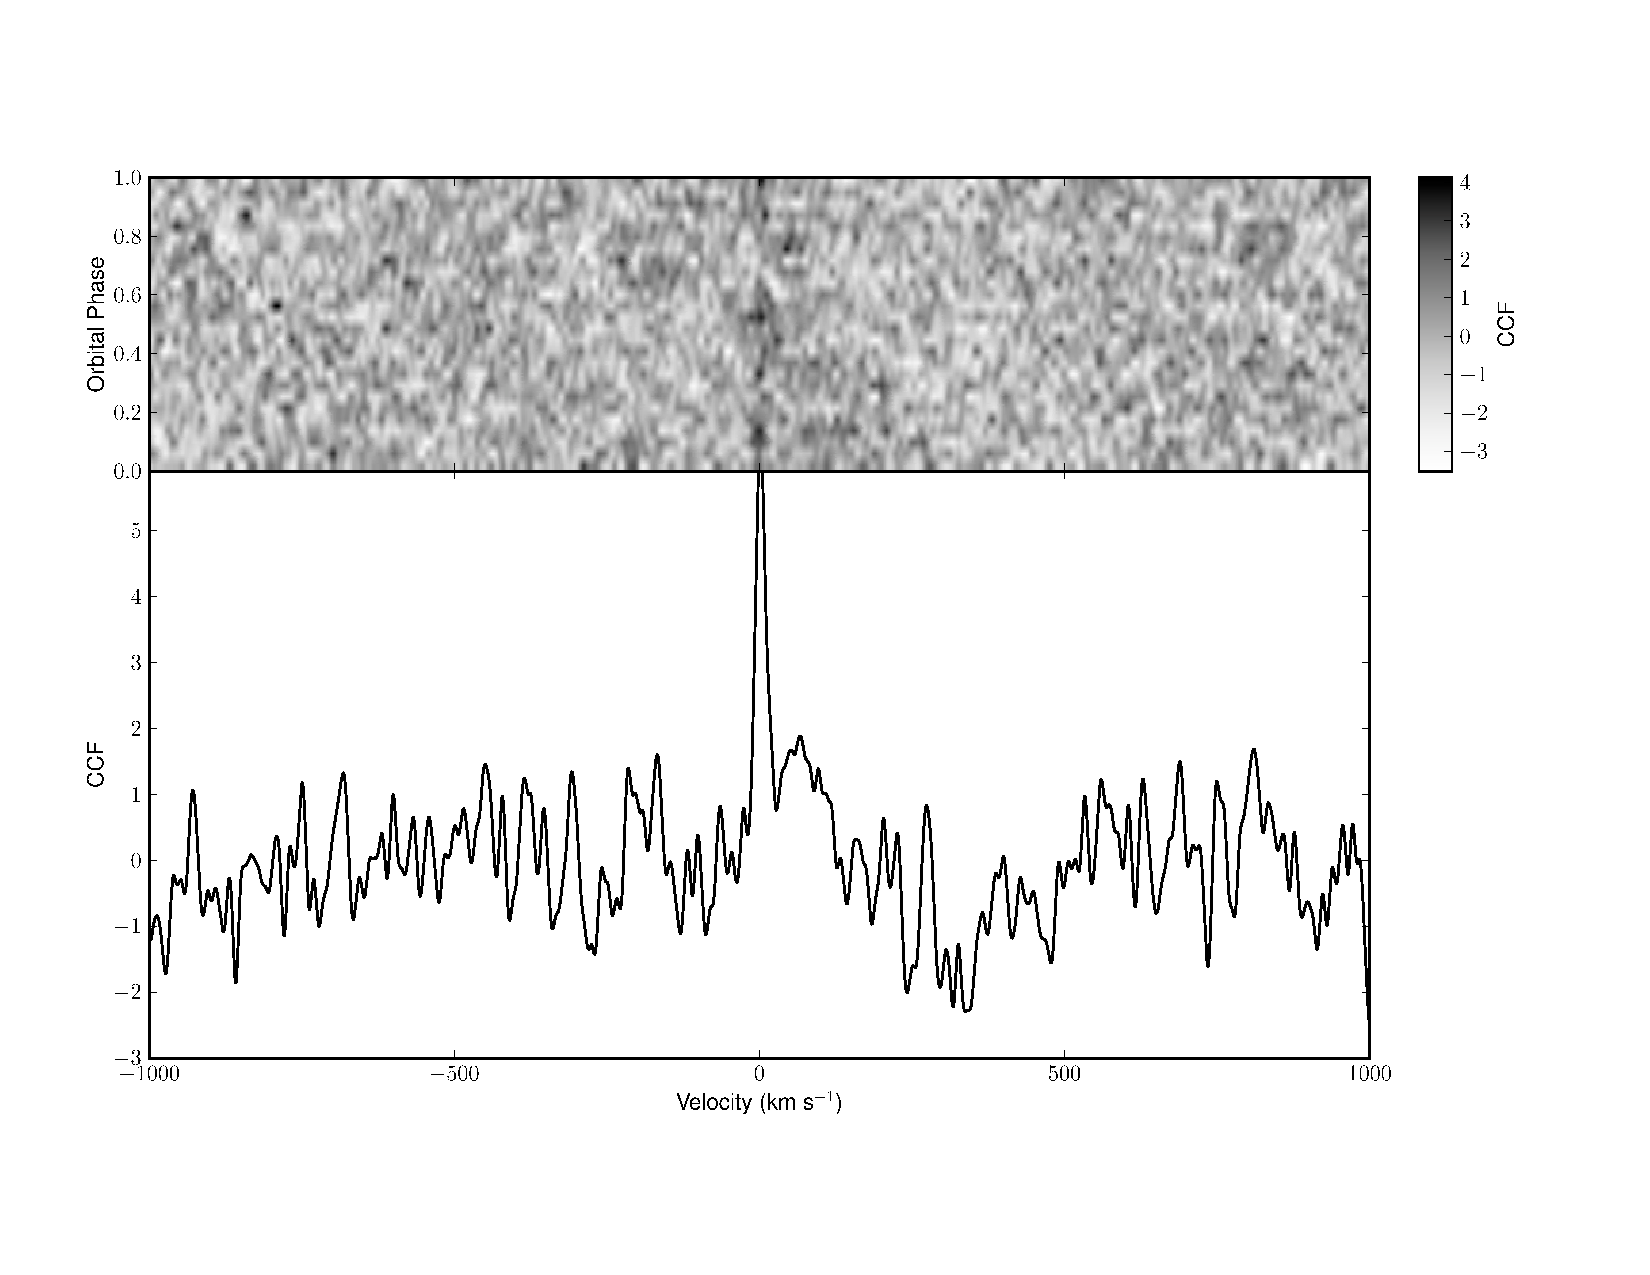
\includegraphics[width=6.5in]{Figures/paper2_fig2.pdf}
  \caption{\emph{Top Panel}: Individual cross-correlation functions for simulations of HD 189733 with an average S/N = 500, and with complete heat redistribution. The velocities are shifted at each orbital phase such that the cross-correlation function should have a peak at 0 km s$^{-1}$; the planet is only detected in a few of the observations. \emph{Bottom panel}: The total cross-correlation function, after adding the cross-correlation functions for each individual observation. Here the planet is very clearly detected with $6.29 \sigma$ significance.}
  \label{paper2_fig:allcorr}
\end{figure}


\begin{figure}[ht]
  \centering
  \includegraphics[width=5.5in]{Figures/paper2_fig3.pdf}
  \caption{A comparison of the HD189733 planet model with the HD209458
  planet model. The gap in the middle is is in between the H and K
  spectral windows, where water absorption in the Earth's atmosphere
  blocks most of the incoming light. HD209458b has a thermal inversion
  in its atmosphere, which generates the emission lines near 1950
  nm. HD189733 b is somewhat cooler and has more water, giving its
  spectrum stronger spectral lines.}
  \label{paper2_fig:modelcomp}
\end{figure}


\begin{figure}[ht]
  \centering
  \includegraphics[width=6.5in]{Figures/paper2_fig4.pdf}
  \caption{A summary of the significance of the point at 0 km s$^{-1}$ in the total cross-correlation functions for each of the mass-ratio guesses, for a series of observations of HD 189733 with an average S/N = 500 and complete heat redistribution (the same as in Figure \ref{paper2_fig:allcorr}). The peak in this figure determines the planet to star mass-ratio, and therefore the true planet mass. The width of the peak $1 \sigma$ below its maximum determines the uncertainty in the planet mass.}
  \label{paper2_fig:massratio}
\end{figure}


%%%%%%%%%%%%%%%%%%%%%%%%%%%%%%%%%%%%%%%%%%%%%%%%%%
% Chapter 5  (B-star pilot study)
%%%%%%%%%%%%%%%%%%%%%%%%%%%%%%%%%%%%%%%%%%%%%%%%%%

\include{paper1}

%%%%%%%%%%%%%%%%%%%%%%%%%%%%%%%%%%%%%%%%%%%%%%%%%%
% Chapter 6  (main survey)
%%%%%%%%%%%%%%%%%%%%%%%%%%%%%%%%%%%%%%%%%%%%%%%%%%


\include{paper6}

%%%%%%%%%%%%%%%%%%%%%%%%%%%%%%%%%%%%%%%%%%%%%%%%%%


%\begin{appendix}

%\chapter{First}
%\lipsum[3]

%\chapter{Second}

%\end{appendix}

\backmatter

\printindex

\cleardoublepage
\phantomsection
%\addcontentsline{toc}{chapter}{Bibliography}
%\chapter*{Bibliography}
%\lipsum[2]
\bibliography{references}

\end{document}
